\documentclass[a4paper,14pt]{extarticle}
\usepackage{geometry}
\usepackage[T2A]{fontenc}
\usepackage[utf8]{inputenc}
\usepackage[french, russian, english]{babel}
\usepackage{amsmath}
\usepackage{amsthm}
\usepackage{amssymb}
\usepackage{fancyhdr}
\usepackage{setspace}
\usepackage{graphicx}
\usepackage{colortbl}
\usepackage{tikz}
\usepackage{pgf}
\usepackage{subcaption}
\usepackage{listings}
\usepackage[colorlinks, linkcolor=blue, urlcolor=blue]{hyperref}
\usepackage{indentfirst}
\graphicspath{{images/}}


\makeatletter
\renewcommand{\@biblabel}[1]{#1.} 
\makeatother

\geometry{left=2.5cm}
\geometry{right=1.5cm}
\geometry{top=1.5cm}
\geometry{bottom=1.5cm}
\renewcommand{\baselinestretch}{1.5}

\newcommand{\bibref}[3]{\hyperlink{#1}{#2 (#3)}}

\renewcommand{\theenumi}{\arabic{enumi}}% Меняем везде перечисления на цифра.цифра
\renewcommand{\labelenumi}{\arabic{enumi}}% Меняем везде перечисления на цифра.цифра
\renewcommand{\theenumii}{.\arabic{enumii}}% Меняем везде перечисления на цифра.цифра
\renewcommand{\labelenumii}{\arabic{enumi}.\arabic{enumii}.}% Меняем везде перечисления на цифра.цифра
\renewcommand{\theenumiii}{.\arabic{enumiii}}% Меняем везде перечисления на цифра.цифра
\renewcommand{\labelenumiii}{\arabic{enumi}.\arabic{enumii}.\arabic{enumiii}.}% Меняем везде перечисления на цифра.цифра

\newcommand{\imgh}[3]{\begin{figure}[h]\center{\includegraphics[width=#1]{#2}}\caption{#3}\label{ris:#2}\end{figure}}

\begin{document}
	\begin{titlepage}
\newpage

\begin{center}
Федеральное государственное автономное образовательное учреждение высшего образования "Национальный исследовательский университет "Высшая школа экономики"
\\
\medskip
Факультет компьютерных наук \\
Основная образовательная программа \\
Прикладная математика и информатика \\
\end{center}

\vspace{8em}

\begin{center}
\Large КУРСОВАЯ РАБОТА \\
\end{center}

\vspace{2em}

\begin{center}
\textsc{\textbf{
Исследовательский проект на тему
\linebreak
"Оценка неопределенности для Машинного Перевода"}}
\end{center}

\vspace{6em}



\newbox{\lbox}
\savebox{\lbox}{\hbox{Ментимер Шаймиев Рудольф Нуриев}}
\newlength{\maxl}
\setlength{\maxl}{\wd\lbox}
\hfill\parbox{17cm}{
\hspace*{5cm}\hspace*{-5cm}Выполнил студент группы 171, 3 курса: \hfill Кузнецов Дмитрий Сергеевич\\
\hspace*{5cm}\hspace*{-5cm}Руководитель КР\hfill 
научный сотрудник Лобачева Екатерина Максимовна\\
%\hspace*{5cm}\hspace*{-5cm}Куратор:\hfill < степень>, <звание>, <ФИО полностью>\\
}


\vspace{\fill}

\begin{center}
Москва 2020
\end{center}

\end{titlepage}% это титульный лист
	\newpage

	{
		\hypersetup{linkcolor=black}
		\tableofcontents
	}

	\newpage
	
	\section{Annotation}
	In the field of machine translation \textit{beam search} is the one of the main methods for improving the quality of the final prediction. However, when using neural network technologies, there is a problem of larger beam size, which limits the richness of beam search. Problem solution will significantly improve the quality of predictions by considering more hypotheses in the process of making predictions. Many factors in the model infrastructure can cause the appearance of the beam problem. In this paper we explore the \textit{larger beam size problem} and its correlation with \textit{model uncertainty}. We also study the propensity of models with an uncertainty estimation to cause beam problem.
	
	\section{Keywords}
		machine translation, uncertainty estimation, beam search, larger beam size problem, model uncertainty
		
	\section{Introduction}
	The task of machine translation is to provide a sentence equivalent in meaning in the target language for the original sentence in the source language. Let $e_1, \dots, e_n$ be a sequence of input sentence tokens' vector representation in the source language. The machine translation model is required to build a sequence of tokens $f_1, \dots, f_n$ in the target language, moreover, in this language, this sequence must have the original meaning.
	
	Most modern models of neuromachine translation follow the paradigm \bibref{seq2seq}{Sutskever et al.}{2014} (seq2seq). Seq2seq models often consist of two recurrent neural networks or groups of networks. One network that processes input tokens is called \textit{encoder}, the second network that builds output predictions is called \textit{decoder}. The encoder task is to encode the input sequence into some hidden representation $h_1, \dots, h_p$, which is fed to the decoder as hidden initialization before building the output prediction. The decoder output is a vector set $\{(p_{i1}, \dots, p_{id})\}_{i=1}^{m}$, where $d$ - target language dictionary power, $m$ - maximum possible prediction sequence length, $p_{ij}$ - the model's confidence that the $i$th token of the predicted sentence will be the $j$th token from the target language dictionary. As a result, the translation model builds a "probability distribution" in the space of the cartesian product of the target dictionary.

	The simplest and most obvious way to build a prediction (final translation) is to select the token that the model is most confident in at each step. If $f_1, \dots, f_m$ is a sequence of model hypotheses' tokens, then $f_i := argmax \, \{p_{ij}\}_{j=1}^{d}$. However, for an optimal prediction $f_1^*, \dots, f_m^*$ it is not always true that in terms of model confidence $f_i^* = argmax \, \{p_{ij}\}_{j=1}^{d}$. This phenomenon is also related to the beam problem, which we will discuss in more detail in the following chapters.
	
	Beam search is used as a more effective solution for building predictions. Its main idea is that instead of selecting the most likely token at each step, we require the model to store $b$ the most likely predictions' prefixes $f_{b1}, \dots, f_{bt}$. Using this approach, we do not choose the locally optimal token, but in general the optimal prefix, which will increase the chances of building a correct prediction.

	It is easy to understand that with the increase of $b$ (this hyperparameter is called \textit{beam size}), the quality of the prediction should also increase, since the number of greedy searches is growing. In practice, it turns out that in neuromachine translation, starting from a certain threshold, the quality decreases significantly with increasing beam size. An illustration of this phenomenon can be seen in Fig. 1. The model used in the experiment is described in the  \bibref{fconv}{Jonas Gehring}{2017}. 
	
	\begin{figure}[t]
		\center{
			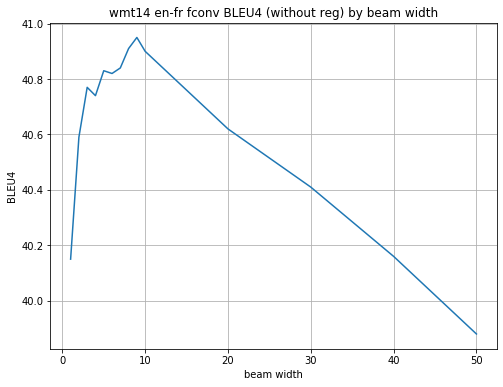
\includegraphics[width=0.7\textwidth]{fconv-bleu4.png}
		}
		\center{\caption{Convolutional Sequence to sequence model BLEU4 evaluation by beam size. Training set: \textit{WMT'14 English-France}}}
	\end{figure}
	
	This problem is called \textit{larger beam size problem}. Next, we will look at the possible causes of this phenomenon in details, until we note that the following situation is not excluded. Suppose on $k_1$ iteration step beam search stores the prefix $f_1, \dots, f_{k_1}$ among $b$ locally optimal, which has the least model confidence among all $b$ prefixes. Let this prefix be constructed in such a way that on the next steps model will find a suffix that complements it in such a way that the final sentence is considered the optimal translation from the model's point of view. There are cases when such a translation can be incorrect. Consider following example. Let us train a translation model on a fairy tale corpus, the source language is Russian and the target language is English. Consider the following sentence: \textit{Жульничество на экзамене однажды может закончиться проблемами}. Suppose following sentence is a model prediction: \textit{At the examination once upon a time}. It is obvious that the meaning of the translation does not correspond to the original sentence, but this sentence is optimal from the point of view of our hypothetical model. Beam problem can cause such situations. The prefix \textit{At the examination once} may have been included in a broad beam search and have been earned a low model confidence. However, due to the fact that we train on a large corpus of fairy tales, where there are many examples of sentences like \textit{Once upon a time...} our model decides that after \textit{Once} it is probably to continue prefix with suffix \textit{upon a time}, which lead to a bad translation.
	
	Note that in the example, some features of the model lead to a bad translation. Our model gave low probable in general predictions as a result under the influence of certain factors. \textit{Uncertainty} can cause such phenomena, in particular \textit{model uncertainty}, the uncertainty of predictions caused by the model. What if we can construct some probability measure on the space of output sentences $f_1, \dots, f_m$. In this case, we will be able to estimate in total how much it is typical to get a particular prediction and adjust the output of the model. The task of explicitly or implicitly constructing such a distribution on outputs is called \textit{uncertainty estimation}.
	
	There are articles that consider different types of uncertainties and their impact on beam search. In this paper, we investigate the influence of model uncertainty on the beam problem. We also investigate the applicability of the uncertainty estimation methods in the neural machine translation problem and their impact on the effectiveness of beam search.
	
	\section{Beam Search}
	\subsection{Method definition}
	Suggest $k$-long prediction prefix:
	\begin{equation}
		f_{:k}^{i} := (f_1^{i}, \dots, f_k^{i}) \text{, \,\, where i - beam search branch index}
	\end{equation}
	
	Let's introduce following iterative method:
	
	\begin{enumerate}
		\item Let's submit a special token of the beginning of the sentence and the encoder hidden state to the decoder input. We get a certain tokens' confidence vector $(p_1^{00}, \dots, p_d^{00})$, where $d$ - target dictionary power.
		
		\item Select $beam$ tokens whose confidence values are $beam$ highest among $ (p_1^{00}, \dots, p_d^{00})$. Here $beam$ is the hyperparameter of the method and is called \textit{beam size}. As a result, we will remember: $f_{:1}^1, \dots, f_{:1}^{beam}$. 
		
		\item In the next iteration, we will submit to the decoder $(f_1^{00}, \dots, f_d^{00})$ as inputs and the hidden state of the previous step. For each token, we get our output distribution $(p_1^{1i}, \dots, p_d^{1i})$ (here $1$ is the iteration number, $i$ is the token number).
		\item For all token $i \in \overline{1, beam}$ consider $\forall j \in \overline{1, d}: \,\, p(f_{:1}^i) * p_j^{1i}$. We get a set of prefixes of length $2$. Let's choose among all $beam * d$ prefixes $beam$ with the greatest confidence. Remember them: $f_{:2}^1, \dots, f_{:2}^{beam}$
		
		\item Iteratively, we will continue the operation $\forall k \in \overline{3, m}$. We will get: $f_ {: k}^1, \dots, f_{:k}^{beam}$
		
		\item As the final prediction select $f_{:m}^i, \dots, f_{:m}^i$ such that its confidence is greatest $\forall i \in \overline{1, beam}$
	\end{enumerate}
	
	In summary, this method stores $beam$ of the "most likely" prefixes at each decoding iteration, in contrast to the naive approach, which greedily selects 1 locally optimal hypothesis at each iteration.
	
	\subsection{Large Beam Size Problem}
	In General, in neuromachine translation tasks large beam size problem is a phenomenon, as a result of which, starting from a certain threshold value, the quality metric decreases with the growth of the beam size. In this section, we will look at some approaches that do not solve the problem completely, but significantly reduce the effect of metric degradation.
	
	The article \bibref{corr_len_bias}{Murray et al.}{2018} raises two issues: the beam problem and the tendency of NMT models to make short predictions. According to the author, solving the short prediction problem involves solving the beam problem.
	
	As a demonstration of the reasons listed in this article that cause the beam problem, consider the following example from the article.
	
	Please refer to Fig.2. Here is a tree of Beam Search predictions for the word \textit{un hélicoptère}. Let the size of the beam search be 2 and on the first iteration we saved two hypotheses: \textit{a} and \textit{an}. Note that all 4 hypotheses can be potential translation options, but \textit{a helicopter} in this example is a correct translation. However, \textit{autogyro} is an only one continuation, thefore the model confidence for this suffix is $1$, and as a result, the model confidence to predict \textit{an autogyro} is equal to $0.4$. At the same time, the probability mass for the \textit{a} continuation suffixes is divided among the words: \textit{helicopter, chopper, whirlybird}. As a result, the confidence for the correct translation of \textit{a helicopter} from the model's point of view is $0.36$. As a result, the model will give a bad prediction. Larger beam size we take, higher probability we get in this situation, hence the loss of quality.
	
	\begin{figure}[t]
		\center{
			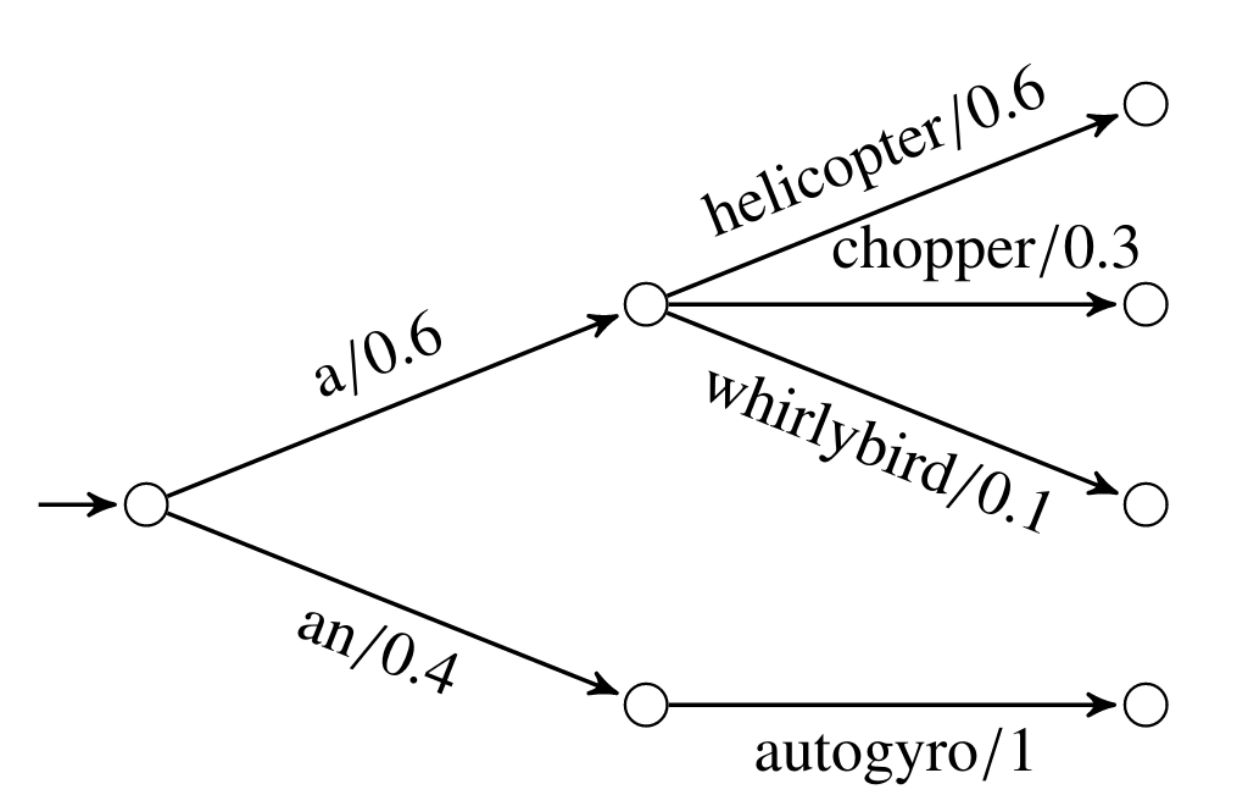
\includegraphics[width=0.5\textwidth]{helicopter.png}
		}
		\center{\caption{Label bias causes this toy word-by-word translation model to translate French helicopter incorrectly}}
	\end{figure}
	
	Note that this example demonstrates the fact that if a certain prefix involves a low-entropy suffix, the model tends to ignore the second input token and predict with high confidence one of several highly probable low-entropy suffixes. As a result, the low entropy of the suffix leads to overestimation of this prediction branch and as a result, poor quality. In addition, there is a high probability of getting short predictions due to low entropy, since the model begins to ignore some tokens in favor of high confidence of low-entropy suffixes. For this reason, the authors of the article consider the short prediction problem and the beam problem together.
	
	Standard quality functional for a machine translation task is \textit{cross-entropy}:
	\begin{equation}
		s(f) = \Sigma_{i=1}^{L}\log p(f_i | f_{:i}), \,\,\, \text{where $L$ - translation length}
	\end{equation}
	
	The authors consider the following quality functional adjustments as solutions:
	\begin{enumerate}
		\item Length normalization
		\begin{equation}
			s'(f) = s(f) / L
		\end{equation}
		
		\item \bibref{gnmt}{Google's NMT system}{2016}. Length normalization. 
		\begin{equation}
			s'(f) = s(f) \Big/ \frac{(5 + L) ^ \alpha}{(5 + 1) ^ \alpha}
		\end{equation}
		
		\item Word reward
		\begin{equation}
			s'(f) = s(f) + \gamma L
		\end{equation}
	\end{enumerate}
	
	Let's look at the results presented in the article for the \textit{WMT'17 Russian-English} model. The architecture presented in the article \bibref{encdec_att}{Bahdanau et al.}{2015} was chosen as the baseline. Appealing to fig.3 we observe that the solution of the short prediction problem using methods proposed above significantly decreases the influence of the beam problem on the considered dataset.
	
	\begin{figure}[t]
		\center{
			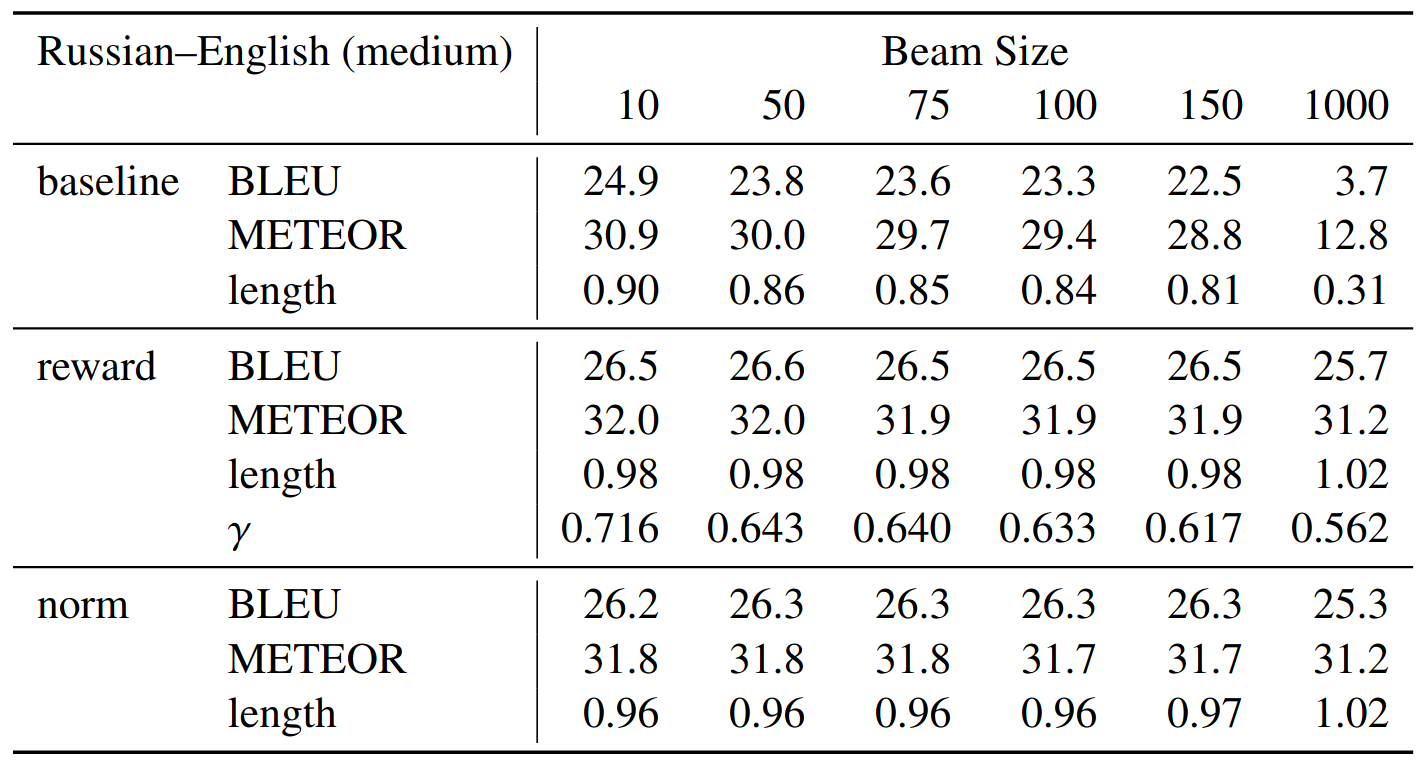
\includegraphics[width=0.7\textwidth]{wmt17_corr.png}
		}
		\center{\caption{Results of Russian-English translation system.}}
	\end{figure}
	
	Let's now look at the article \bibref{six_chall}{Koehn et al.}{2017}. This is a review article on the main problems of neuromachine translation, including the beam problem.
	
	\begin{figure}[t]
		\center{
			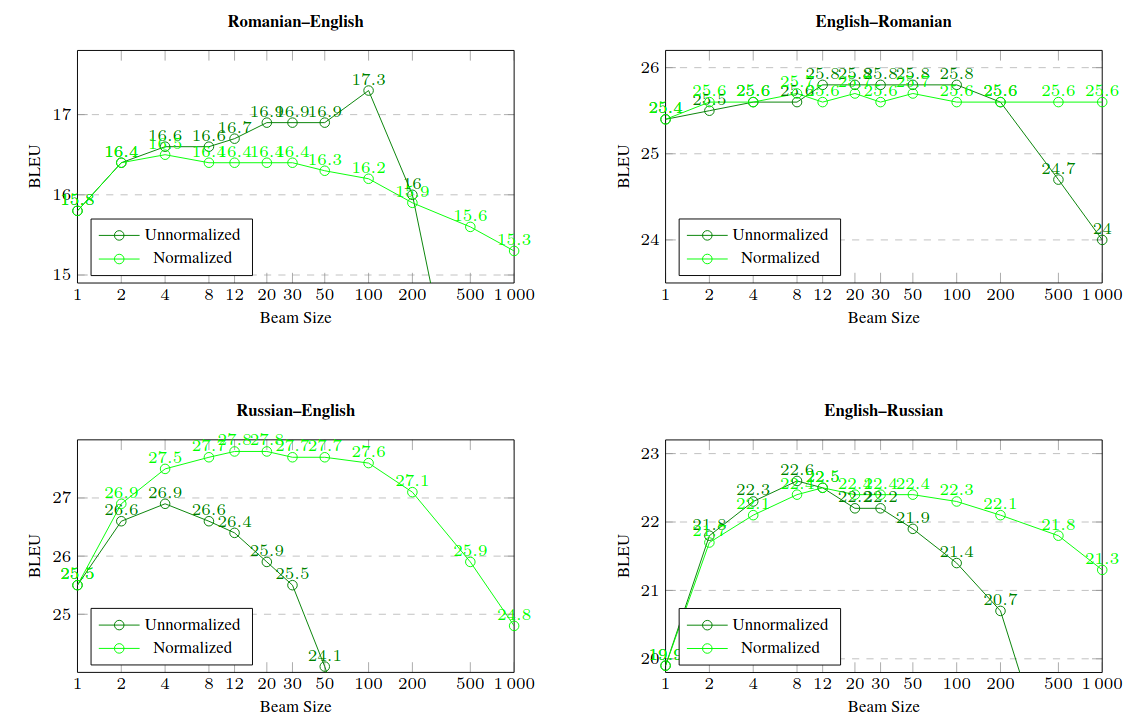
\includegraphics[width=0.8\textwidth]{six_chall_graph.png}
		}
		\center{\caption{Translation quality with varying beam sizes. For large beams, quality decreases, especially when not normalizing scores by sentence length.}}
	\end{figure}
	
	The authors of the article do not present new solutions for the problem, but conduct a review study. As a baseline, they use the same neural network as in the previous article: attention-based encoder-decoder. Fig. 4 presents their results for various \textit{WMT} datasets. Here, normalization is the Length normalization from the previous article.
	
	The results obtained in this article are consistent with the results and conclusions of the previous article.
	
	Consider an article that offers a different method for solving the problem \bibref{calibration}{Kumar et al.}{2019}.

	In this article the beam problem solution is based on the calibration of the probability distribution $p_{it}: = p(f_{i, t} | f_{i,:t})$, here $i$ is the index of the sample example. Before starting the review, let's introduce the definition of "well-calibrated" distribution. Output distribution $p (f_{i, t} | f_{i, :t})$ \textit{well calibrated} if:
	\[
		\forall \beta \in [0, 1]: \frac{ | \{ y \in V |\, p(y) = \ beta \} | }{d}=\beta
	\]
	where V is the target language dictionary.
	
	Let's denote calibration metrics \textbf{expected calibration error (ECE)}:
	
	Let $\mathbf{x}_i$ reference sentece is $\mathbf{y}_i = (y_{i1}, \dots, y_{im})$.
	
	Model predictions: $\mathbf{f}_{it} := argmax_{f} p(f | f_{i, :t})$.
	
	$C_{it}(f) := \delta(y_{it} = f)$, where $\delta$ - Kronecker delta.
	
	Let's divide probability space $[0, 1]$ by $M$ equal bins: $I_1, \dots, I_M$.
	
	Let $L = \sum_i^N |\mathbf{y}_i|$ be a total output token length.
	
	Then:
	\begin{equation}
		ECE = \frac1{L}\sum_{b=1}^{M}\Big|\sum_{i, t:\, p(\mathbf{f}_{it}) \in I_b} C_{it}(\mathbf{f}_{it}) - p(\mathbf{f}_{it})\Big|
	\end{equation}
	
	The reasons why the probability distribution calibration can solve problems with beam size follow from the examples we discussed above.
	
	The authors consider the classic \textit{temperature scaling as the basic method}:
	
	The method is quite simple. It is necessary to raise all probability distribution to the power of $\frac1{T}$, where $T$ is the hyperparameter of the method:
	\[
		p_{it} \rightarrow p_{it}^{\frac1{T}}
	\]
	
	This approach does not change the relative values of probabilities, i.e. it does not locally change the optimality of a particular choice, but it helps to smooth out the consequences of overestimating or underestimating certain prefixes or suffixes.
	
	\begin{figure}[t]
		\center{
			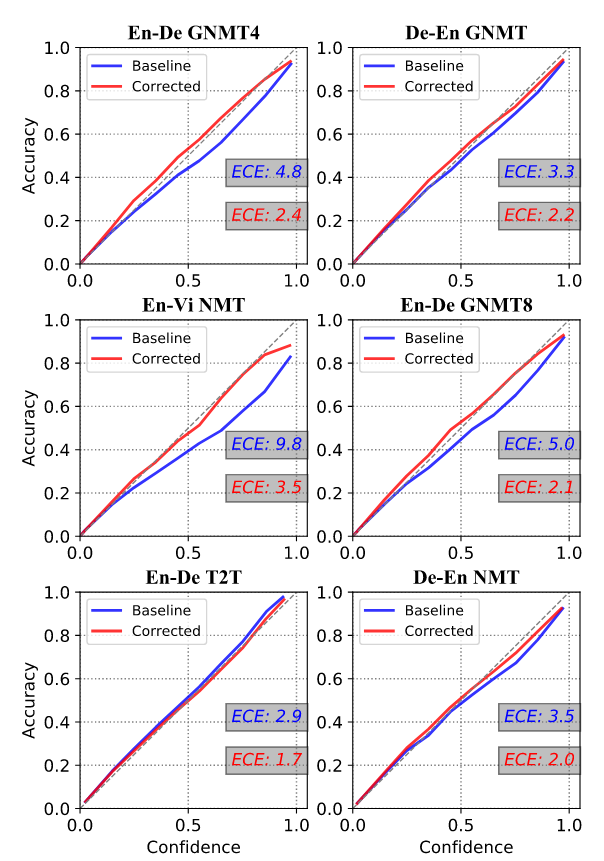
\includegraphics[width=0.4\textwidth]{tscaling.png}
		}
		\center{\caption{Reliability Plots for various baseline models on the test sets along with their ECE values(Blue).The x-axis is expected confidence after binning into 0.05 sized bins and y-axis is accuracy in that confidencebin.  Reliability plots for calibrated (corrected) models (Red).  ECE values in corresponding colors.  Test setsare mentioned in the corresponding references.}}
	\end{figure}
	
	The authors consider 3 models trained on \textit{WMT} as a baseline: \bibref{encdec_att}{attention-based encoder-decoder}{2015}, GNMT \bibref{gnmt}{Wu et al.}{2016}, transformer \bibref{transformer}{Vaswani et al.}{2017}. Fig. 5 shows the probability plot for different models. Here, the classic \textit{temperature scaling} is used as a calibration method.
	
	In order not to overweight the literary review, we will not formally introduce the method proposed by the authors. We will consider conceptual differences from the default temperature scaling. To study the formal definition of the method, you can refer to the article \bibref{calibration}{Kumar et al.}{2019}.
	
	As a result of experiments, the authors found out that end of sequence (EOS) token probability is the worst calibrated among all other tokens. Therefore, first of all, the authors calibrate the distribution of the EOS token. This observation strongly correlates with the conclusions from the articles reviewed earlier. In contrast to the classic temperature scaling and the hyperparameter selection on a validation set, the authors propose to make the hyperparameter flexible, different for each example and token index, i.e. not to smooth the entire probability mass, but to smooth it depending on the offset of the probability density on the token. To find the values of hyperparameters, it is proposed to use two fully connected two-layer neural networks with 3 neurons on the hidden layer. The composition of two neural networks with optimization \textit{Negative Log Likelihood (NLL)} is proposed to train to predict the value of the hyperparameter $T$ for a given example and a token in the prediction.
	
	On fig.6 you can observe ECE for different calibration methods. It can also be seen that the authors' calibration method achieves the best results on the most part of the baseline models from the BLEU point of view.
	
	\begin{figure}[t]
		\center{
			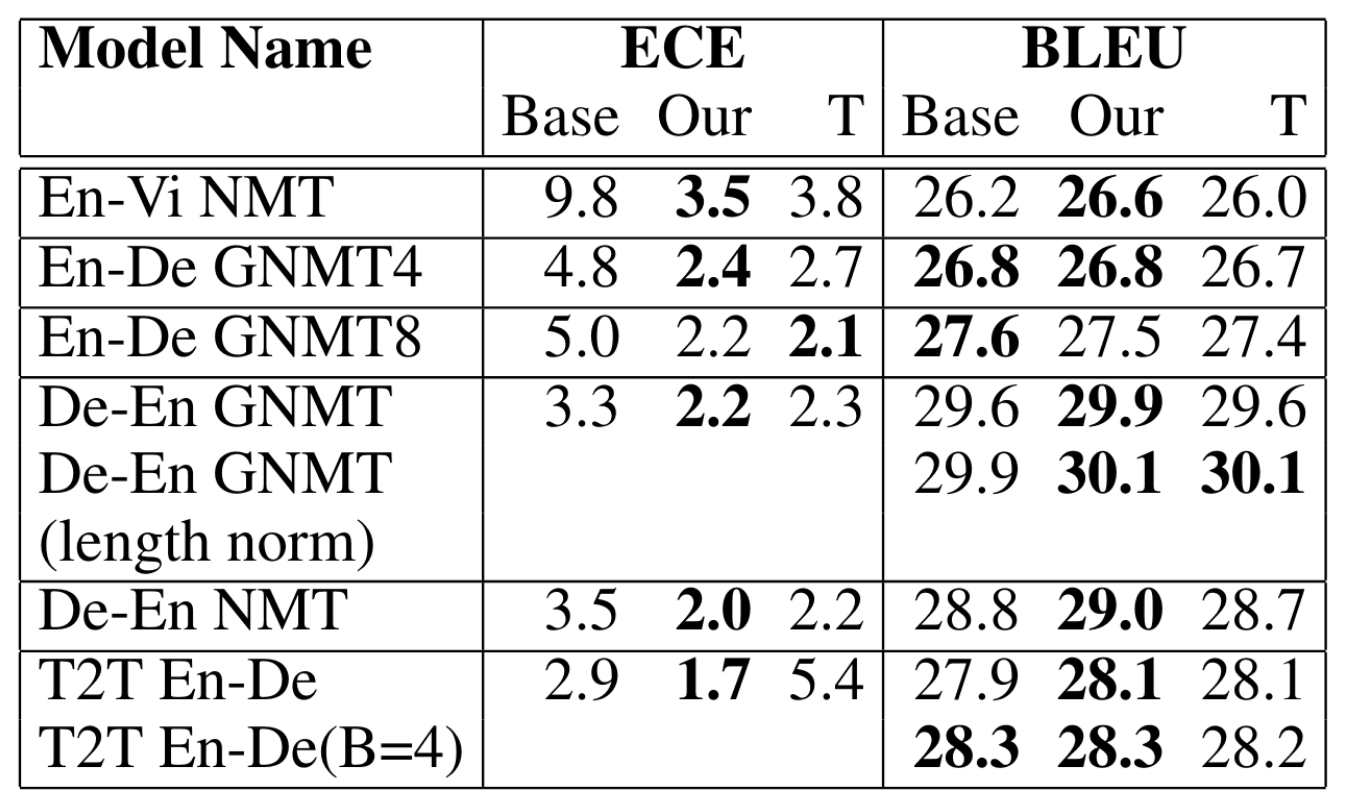
\includegraphics[width=0.6\textwidth]{ece_calibration.png}
		}
		\center{\caption{Expected Calibration Errors on test data of baseline and models calibrated by two different methods.BLEU is without length normalization, except in De-En GNMT. \textit{Our} - Authors' calibration method, \textit{T} - temperature scaling.}}
	\end{figure}
	
	Now, turning to Fig.7, let's look at the effect of the authors' calibration on the beam size problem. It is easy to see that calibration significantly reduces the impact of the beam problem.
	
	\begin{figure}[t]
		\center{
			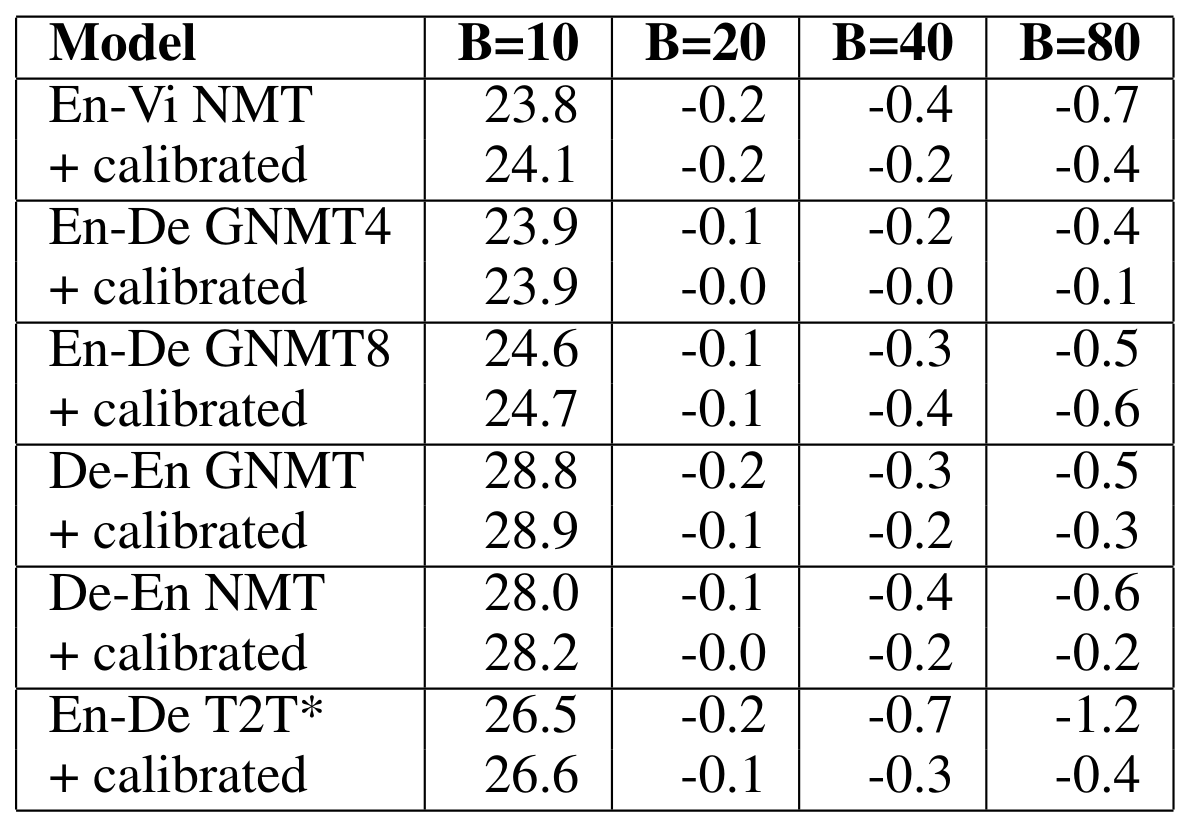
\includegraphics[width=0.6\textwidth]{beam_calibration.png}
		}
		\center{\caption{BLEU with increasing beam on the devset. *Beam sizes for Transformer/T2T: 4, 8, 10 and 12}}
	\end{figure}
	
	In this section, we investigated the possible causes of the beam problem, as well as methods of counteraction. Unfortunately, it is not possible to draw unambiguous conclusions from the results of the article about which method shows the best results due to the fact that the experiments in the articles were carried out in different configurations. According to approximate estimates, both methods show good results, are easy to implement, but do not solve the problem completely.
	
	In the next section, we look at a different view of the beam problem, from the perspective of uncertainty.
	
	\section{Uncertainty}
	\subsection{Definition}
	This information was obtained from the article \bibref{prior}{Malinin et al.}{2018}
	
	Uncertainty in machine learning is usually understood as a measure of the nondegeneration of the distribution on the model predictions at a fixed input. Less formally, if we were able to estimate uncertainty, we could tell how much we can trust the model's predictions.
	
	There are several types of uncertainties: data uncertainty, model uncertainty, and distributive uncertainty. \textit{Data uncertainty (aleatoric uncertainty)} - type of uncertainty caused by the nature of the data, including noise, class balance, etc. \textit{Model uncertainty (epistemic uncertainty)} - measures the uncertainty in estimating the model parameters given the training data - this measures how well the model is matched to the data. Model uncertainty is reducible as the size of training data increases. \textit{Distributional uncertainty} arises due to mismatch between the training and test distributions. 
	
	It is important for the model to evaluate all types of uncertainty, because they are caused by different reasons and have different negative effects.
	
	\subsection{Analyzing Uncertainty in Neural Machine Translation}
	In the article \bibref{anal_uncertainty}{Ott et al.}{2018} \textit{data uncertainty} is being investigated.
	
	Let's introduce several base definition from the article. \textit{Intrinsic uncertainty} is the result of existence of several semantically equivalent translations of the same source sentence, for instance there are several ways to express the same meaning. There are also sources of uncertainty due to \textit{under-specification} when translating into a target language more inflected than the source language. Without additional context, it is often impossible to predict the missing gender, tense or number. \textit{Extrinsic uncertainty} is the result of addition low quality web crawled data. For example, authors notice that there are between 1.1\% to 2.0\% samples in  WMT’14 En-De and WMT’14 En-Fr datasets, in which training example is a copy of a source sentence.
	
	The architecture described in the article \bibref{fconv}{Gehring et al.}{2017} is specified as the baseline of the experiments.
	
	One of the main problems that is raised in this article is an effect of \textit{uncertainty} on the degradation of quality with the growth of beam size. Authors notices copies (extrinsic uncertainty) are overrepresented in the output of beam search. On WMT'14 En-Fr, beam search outputs copies at the following rates: 2.6\% (beam=1), 2.9\% (beam=5), 3.2\% (beam=10) and 3.5\% (beam=20).
	
	\begin{figure}[t]
		\center{
			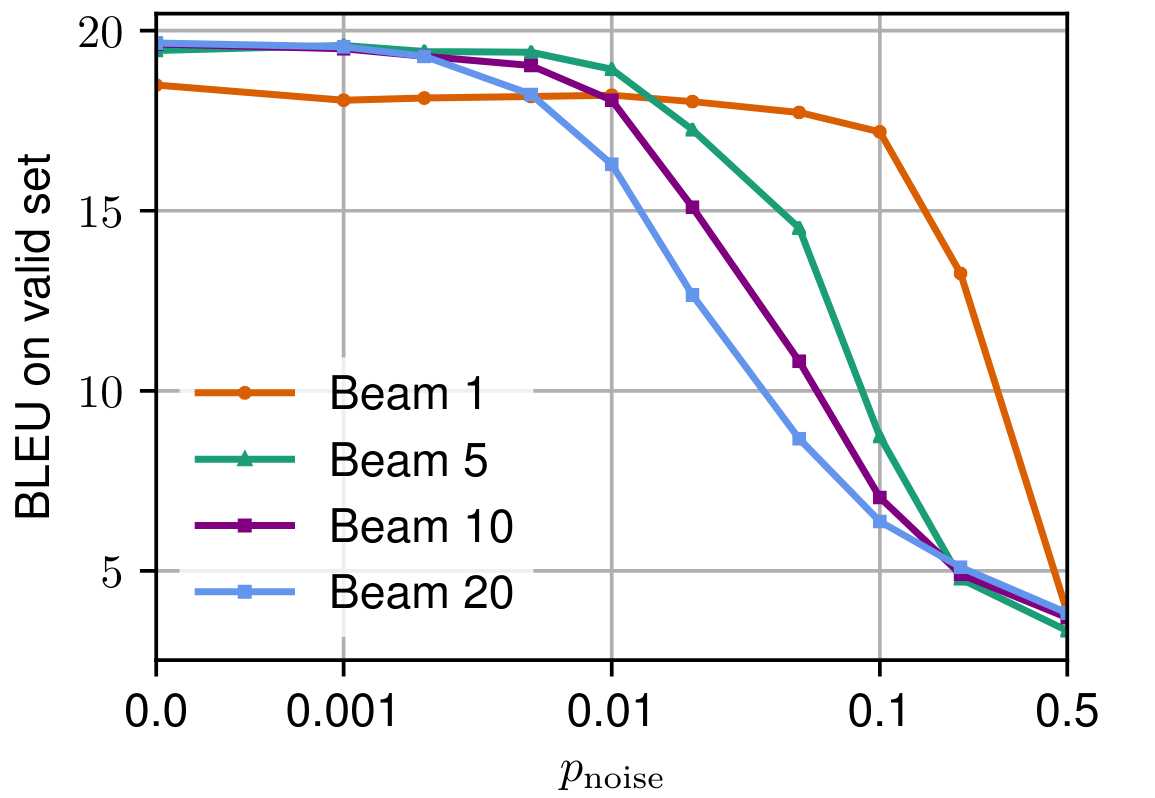
\includegraphics[width=0.6\textwidth]{unc_beam_noise.png}
		}
		\center{\caption{Translation  quality  of  models  trained  on  WMT’17 English-German news-commentary data with added synthetic copynoise in the training data (x-axis) tested with various beam sizeson the validation set.}}
	\end{figure}
	
	The authors conducted an experiment, the results of which can be seen in Fig. 8, in which WMT'17 added explicitly replaced random examples from the training with copies of the original sentence. It is clearly seen that this leads to quality degradation with increasing noise. Moreover, models with a larger beam size suffer more from extrinsic uncertainty, which confirms the thesis put forward in the previous paragraph.
	
	\begin{figure}[t]
		\center{
			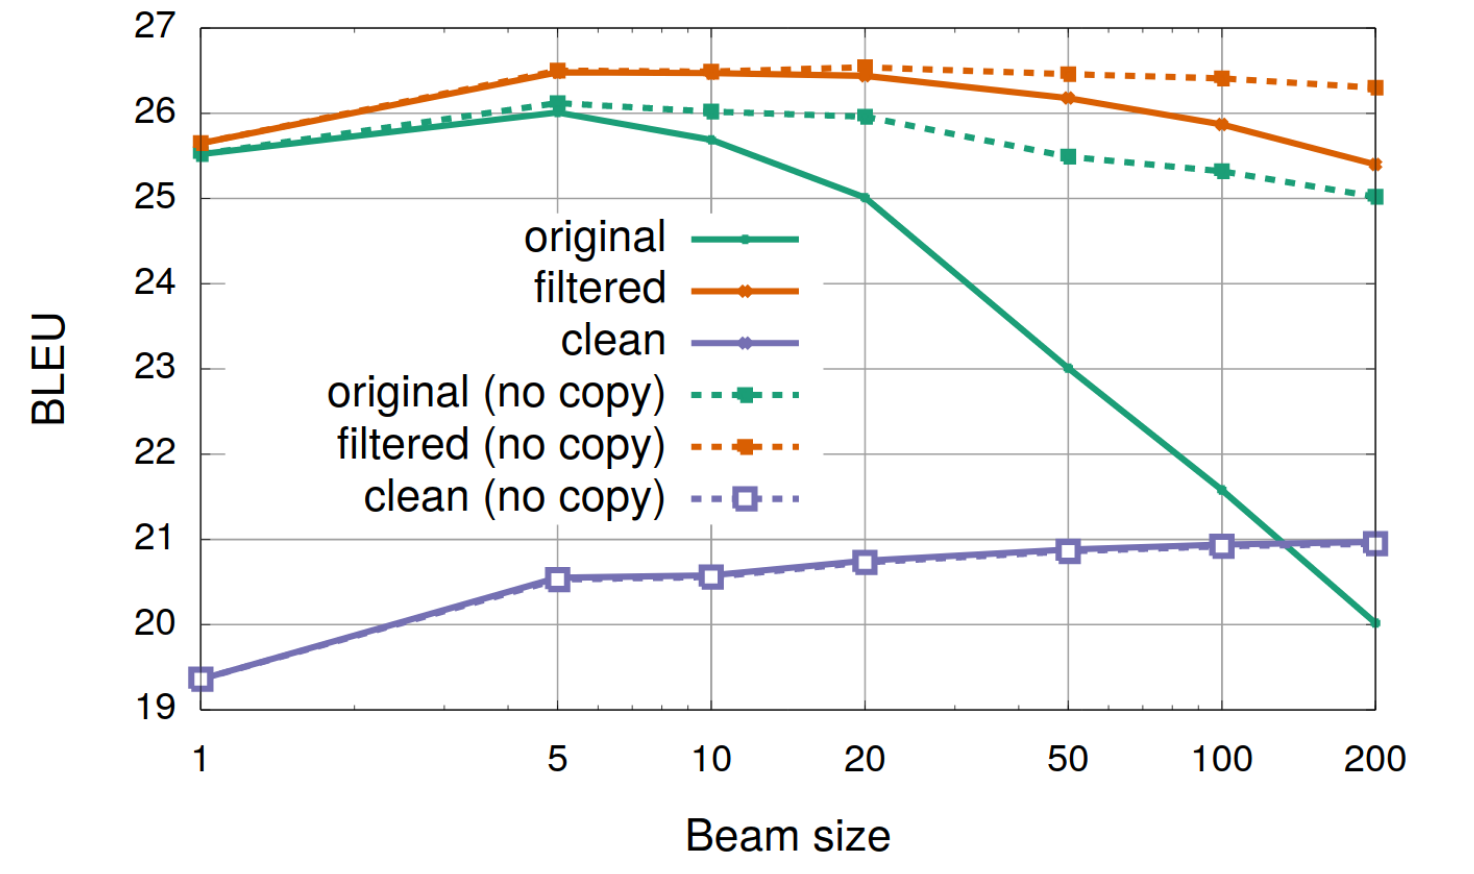
\includegraphics[width=0.6\textwidth]{unc_beam_meth.png}
		}
		\center{\caption{BLEU on newstest2017 as a function of beam width for models trained on all of the WMT’17 En-De training data (original), a filtered version of the training data (filtered) and a small but clean subset of the training data (clean). They also show results when excluding copies as a post-processing step (no copy).}}
	\end{figure}
	
	The authors suggest two approaches to preparing data for training. First, they pre-process the training data by removing low scoring sentence-pairs according to a model trained on the news-commentary portion of the WMT’17 English-German data (filtered). Second, they apply an inference con-straint that prunes completed beam search hypotheses whichoverlap by 50\% or more with the source (no copy). The results can be seen in Fig. 9. They are fully consistent with the conclusions obtained earlier.
	
	\section{Work Plan}
	We have studied the analysis of the raised problems and the existing solutions at the moment of work writing. The purpose of this work is to investigate the influence of \textit{model uncertainty} on the larger beam size problem, and to try to apply existing methods in the field of \textit{uncertainty estimation} in the problem of neuromachine translation.
	
	The course work will be based on the following plan:
	\begin{enumerate}
		\item Study and analysis state-of-the-art models of neuromachine translation. Their applicability to the problem.
		\item Selecting the appropriate set of training cases for problem analysis
		\item Experiments results from the reviewed articles validation with different beam sizes on our own configurations.
		\item Analysis of the results of the experiments from the point of view of uncertainty. Comparison of predictions for different beam sizes at the level of the beam search tree.
		\item Research of existing solutions in the field of Uncertainty estimation
		\item Selecting a set of potentially effective models for uncertainty estimation
		\item Conducting experiments to study the effect of uncertainty estimation on the beam problem with models from a potentially effective set.
		\item Implementation of the final configuration
		\item Final test
		\item Course work writing complition
	\end{enumerate}
	
	\begin{thebibliography}{0}		
		\bibitem{fconv}\hypertarget{fconv}{}
		\href{https://arxiv.org/pdf/1705.03122.pdf}
		{Jonas Gehring, Michael Auli, David Grangier, Denis Yarats, Yann N. Dauphin. Facebook AI Research. Convolutional Sequence to Sequence Learning. 25 Jul 2017.}
		
		\bibitem{seq2seq}\hypertarget{seq2seq}{}
		\href{https://papers.nips.cc/paper/5346-sequence-to-sequence-learning-with-neural-networks.pdf}
		{Ilya Sutskever, Oriol Vinyals, Quoc V.Le. Sequence to Sequence Learning with Neural Networks. Google. 10 Sep 2014.}
		
		\bibitem{encdec_att}\hypertarget{encdec_att}{}
		\href{https://arxiv.org/pdf/1409.0473.pdf}
		{Dzmitry Bahdanau, KyungHyun Cho, Yoshua Bengio. Neural Machine Translation by Jointly Learning to Align and Translate. 19 May 2016.}
		
		\bibitem{corr_len_bias}\hypertarget{corr_len_bias}{}
		\href{https://arxiv.org/pdf/1808.10006.pdf}
		{Kenton Murray, David Chiang. Department of Computer Science and Engineering, University of Notre Dame. Correcting Length Bias in Neural Machine Translation. 31 Aug 2018.}
		
		\bibitem{gnmt}\hypertarget{gnmt}{}
		\href{https://arxiv.org/pdf/1609.08144.pdf}
		{Yonghui Wu, Mike Schuster, Zhifeng Chen, Quoc V. Le, Mohammad Norouzi. Google’s Neural Machine Translation System: Bridging the Gapbetween Human and Machine Translation. 8 Oct 2016}
		
		\bibitem{transformer}\hypertarget{transformer}{}
		\href{https://arxiv.org/pdf/1706.03762.pdf}
		{Ashish Vaswani, Noam Shazeer, Niki Parmar, Jakob Uszkoreit, Llion Jones, Aidan N. Gomez, Lukasz Kaiser. Attention Is All You Need. 6 Dec 2017.}
		
		\bibitem{six_chall}\hypertarget{six_chall}{}
		\href{https://arxiv.org/pdf/1706.03872.pdf}
		{Philipp Koehn, Rebecca Knowles. Six Challenges for Neural Machine Translation. 12 Jun 2017.}
		
		\bibitem{calibration}\hypertarget{calibration}{}
		\href{https://arxiv.org/pdf/1903.00802v1.pdf}
		{Aviral Kumar, Sunita Sarawagi. Calibration of Encoder Decoder Models for Neural Machine Translation. 3 Mar 2019.}
		
		\bibitem{anal_uncertainty}\hypertarget{anal_uncertainty}{}
		\href{https://arxiv.org/pdf/1803.00047.pdf}
		{Myle Ott, Michael Auli, David Grangier, Marc'Aurelio Ranzato. Analyzing Uncertainty in Neural Machine Translation. 13 Aug 2018.}
		
		\bibitem{prior}\hypertarget{prior}{}
		\href{https://papers.nips.cc/paper/7936-predictive-uncertainty-estimation-via-prior-networks.pdf}
		{Andrey Malinin, Mark Gales. Predictive Uncertainty Estimation via Prior Networks. NeurIPS 2018.}
	\end{thebibliography}


\end{document}

